% vim:ts=4:sw=4
% Copyright (c) 2014 Casper Ti. Vector
% Public domain.

\def\qui {1E 1547-54}
\def\uu {4U~0142$+$61}
\def\oo {1E~1048$-$59}
\def\kes {1E~1841$-$045}
\def\axj {AX~J1845$-$02}
\def\rxs {1RXS~J1708$-$40}
\def\eee {1E~2259$+$586}
\def\xte {XTE~J1810$-$197}
\def\cxo {CXOU~J1647$-$45}
\def\smc {CXOU~J0100-72}
\def\zerosei {SGR~1806$-$20}
\def\zerozero {SGR~1900$+$14}
\def\sedici {SGR~1627$-$41}
\def\lmc {SGR~0526$-$66}
\def\quil {1E 1547.0-5408}
\def\uul {4U~0142$+$61}
\def\ool {1E~1048$-$586}
\def\kesl {1E~1841$-$045}
\def\axjl {AX~J1844.8$-$0256}
\def\rxsl {1RXS~J170849$-$400910}
\def\eel {1E~2259$+$586}
\def\xtel {XTE~J1810$-$197}
\def\cxol {CXOU~J164710.2$-$455216}
\def\smcl {CXOU~J010043.1-721134}

\chapter{X射线波段的研究}

\section{反常X射线脉冲星和软伽马射线重复爆的硬X射线辐射}

反常X射线脉冲星(Anomalous X-ray pulsars,AXPs)和软伽马射线重复爆(soft gamma-ray 
repeaters,SGRs)是两类特殊的脉冲星类致密天体。AXPs是首先作为软X射线源被
发现的($<$10\,keV)\supercite{fg81,scs86,ims94},而SGRs则是因为其在
硬X射线波段的短爆发现被发现的\supercite{mgg+79,mgi+79}。我们探测到了SGRs的持
续X射线辐射,也发现了AXPs有爆发现象,因此现在普遍认为
AXPs和SGRs是同一类脉冲星类致密天体\supercite{m08}。
%
经过十多年的多波段的观测和研究,我们发现了AXPs和SGRs的多种
多样的现象。在这一类天体背后的极端的天体物理环境吸引了众多天体物理学家的
目光\supercite{m08}。

AXPs和SGRs最主要的两个特征是没有伴星的证据和X射线光度
大于自转能损。这两个特征将AXPs和SGRs与其他X射线脉冲星
区分开来。AXPs和SGRs有很多相同点,比如相似的自转周期
和自转周期的导数、比较窄的自转周期的分布、没有射电辐射以及与超新星遗迹成携等等。
表\ref{tab-list1}和\ref{tab-list2}列出了现在已知的AXPs和SGRs\supercite{m08}。

%%%%%%%%%%%%%%%%%%%%%%%%%%%%%%%%%%%%%%%%%%%%%%%%%%%%%%%%%%%%%%%%%%%%%%%%%%%%%%%%%%%%
\begin{table}
\caption{目前已知的反常X射线脉冲星~\supercite{m08}。}
 \centering
\label{tab-list1}
\begin{tabular}{lcccc}
\hline\noalign{\smallskip}
Name           &Hard X-rays$^{(a)}$& Soft X-rays$^{(a)}$          & Distance      & Location \\[3pt]
               &  ($>$10 keV)      & ($<$10 keV)                  & (kpc)         &  \\[3pt]
\hline
\multicolumn{5}{c}{\textbf{Anomalous X--ray Pulsars}}\\ [3pt]
 \hline
\smc           & -                 & P                            &  61           & SMC \\[3pt]
\cite{lfmp02}  &                   & \cite{lfmp02}                &               &     \\[3pt]
 \hline
\uu            & P                 & P                            &  3.6          &     \\[3pt]
\cite{ms95}    & \cite{dhk+06}     & \cite{ims94}                 &\cite{dv06a}   &     \\[3pt]
\hline
\oo            & D                 & P                            & 9             &     \\[3pt]
\cite{ms95}    & \cite{lwr08}      & \cite{scs86}                 &\cite{dv06a}   &     \\[3pt]
\hline
\qui           & -                 & P,T                          & 9             & SNR G327.24--0.13 \\[3pt]
\cite{gg07}    &                   & \cite{hgr+08}                &\cite{ccr+07}  &     \\[3pt]
\hline
\cxo           &     -             & P,T                          & 3.9           & Massive Star Cluster \\[3pt]
\cite{mcc+06}  &                   &\cite{mcc+07}                 &\cite{kd07}    &  Westerlund 1     \\[3pt]
\hline
\rxs           & P                 & P                            & 3.8           &      \\[3pt]
\cite{snt+97}  & \cite{khd+06}     &\cite{snt+97}                 &\cite{dv06a}   &      \\[3pt]
\hline
\xte           & -                 & P,T                          & 3.1           &      \\[3pt]
\cite{ims+04}  &                   &\cite{ims+04}                 &\cite{dv06a}   &      \\[3pt]
\hline
\kes           & P                 & P                            & 8.5           & SNR Kes 73\\[3pt]
\cite{vg97}    & \cite{khm04}      & \cite{vg97}                  & \cite{tl08}   &     \\[3pt]
\hline
\axj $^{(b)}$  & -                 & P,T                          & 8.5           & SNR G29.6+0.1 \\[3pt]
\cite{tkk+98}  &                   & \cite{tkk+98}                & \cite{tkk+98} &     \\[3pt]
\hline
\eee           & -                 & P                            & 7.5           & SNR CTB 109 \\[3pt]
\cite{ms95}    &                   &\cite{fg81}                   & \cite{dv06a}  &     \\[3pt]
\hline
 \hline
\end{tabular}
\end{table}

%%%%%%%%%%%%%%%%%%%%%%%%%%%%%%%%%%%%%%%%%%%%%%%%%%%%%%%%%%%%%%%%%%%%%%%%%%%%%%%%%%%%
\begin{table}
\caption{目前已知的软伽马射线重复爆~\supercite{m08}。}
 \centering
\label{tab-list2}
\begin{tabular}{lcccc}
\hline\noalign{\smallskip}
Name           &Hard X-rays$^{(a)}$& Soft X-rays$^{(a)}$          & Distance      & Location \\[3pt]
               &  ($>$10 keV)      & ($<$10 keV)                  & (kpc)         &  \\[3pt]
\hline
\multicolumn{5}{c}{\textbf{Soft Gamma-ray Repeaters}} \\ [3pt]
 \hline
\lmc           & -                 & P                            & 55            & LMC, SNR N49 \\[3pt]
\cite{cdp+80}  &                   & \cite{rkl94}                 &               &     \\[3pt]
\hline
\sedici        & -                 & D,T                          & 11            & \\[3pt]
\cite{wkv+99}  &                   & \cite{wkv+99}                & \cite{ccdd99} &     \\[3pt]
\hline
\zerosei       & D                 & P                            & 15            & Massive Star Cluster \\[3pt]
\cite{lff+86}  &\cite{mgm+05}      &\cite{kds+98}                 & \cite{ce04}   &     \\[3pt]
\hline
\zerozero      & D                 & P                            & 15            & Massive Star Cluster \\[3pt]
\cite{mgg+79}  & \cite{gmt+06}     &\cite{hkw+99}                 & \cite{vhl+00} &     \\[3pt]
\hline
 \hline
\end{tabular}

\textbf{Notes:}

$^{(a)}$ D = detection; P = pulsations detected; T = transient

$^{(b)}$ Candidate AXP (no $\dot P$ measurement)
\end{table}

\subsection{谱的性质}

尽管AXPs和SGRs的距离很难精确地确定,但是粗略的估计可以
通过X射线的吸收和与它们成携的超新星遗迹的距离得到。典型的距离在至少几个kpc的量级,
意味着典型的光度在$10^{34-36}$\,$\rm{erg\ s^{-1}}$的量级。这样的X射线光度
远大于从自转周期和自转周期导数得到的自转能损。

AXPs在10\,keV以下有比较软的谱,并且能被一个比较陡的幂律谱(光子指数$\sim3-4$)
和一个黑体谱拟合($kT\sim0.5$\,keV)。SGRs在10\,keV以下的谱通常
比AXPs的硬,能很好地用一个光子指数为$\sim2$的幂律谱拟合。人们也
尝试了用两个黑体谱来拟合AXPs的谱\supercite{m08,hg05},并且发现了
在高质量的SGRs的谱中的类似黑体的成分\supercite{m08,mte+05,met+06}。
这些结果暗示AXPs和SGRs的软X射线辐射可能是热辐射,而
总的能谱远比一个黑体谱复杂\supercite{m08}。

AXPs和SGRs的硬X射线辐射是首先被INTEGRAL卫星发现的\supercite{khm04,dhk+06,mgm+05,gmt+06}。
考虑到AXPs在10\,keV以下的较软的谱,这是很让人吃惊的发现。更让人惊讶
的是在20\,keV以上AXPs的谱比软硬,而SGRs的谱则比较软。在
硬X射线波段比较平的谱说明AXPs和SGRs在硬X射线波段的
辐射占了总辐射能量的很大一部分。硬X射线辐射的起源目前还不清楚,我们将在后面
详细讨论。

\subsection{爆发现象的性质}

短爆发(short bursts)是SGRs的标志性特征,也是发现这一类有极端
天体的特征。在活跃期内,SGRs在硬X射线波段重复地产生短爆发。
短爆发的峰值流量能够达到$\sim10^{42}$\,$\rm{erg\ s^{-1}}$,持续时间大约为
$0.01-1$\,s。大部分的爆发都是由一个或者多个脉冲组成的,这些脉冲都呈现快速
上升、缓慢下降的特征。短爆发的谱在15\,keV以上能被一个光薄的热韧致辐射模型
拟合($kT\sim30-40$\,keV),但是这个模型在低能段($\sim1-2$\,keV)就不能拟合
了\supercite{flu94}。为了能拟合宽能量范围内的谱(1到100\,keV),之前的工作使用了
两个黑体辐射的模型,一个黑体的温度是$kT_{\rm{1}}\sim2-4$\,keV,另一个黑体
的温度是$kT_{\rm{2}}\sim8-12$\,keV\supercite{fcm+04}。来自AXPs的
短爆发是被RXTE卫星发现的\supercite{klc00,kgw+03},这进一步证实了AXPs和SGRs是同一类天体。

比短爆发更剧烈的现象是SGRs的巨爆发(giant flares),这种爆发
现象释放的能量在$\sim(2-500)\times10^{44}$\,ergs的量级。目前为止共观测到三个巨爆发,
都是来自于SGRs\supercite{m08}。巨爆发的典型特征是一个很短很硬的
尖峰,之后是一个很长的、脉冲的尾巴。巨爆发的峰值流量能达到$10^{47}$\,$\rm{erg\ s^{-1}}$
的量级。爆发的峰的上升时间短于几个毫秒,而持续时间一般是几十秒。峰的谱比一般
的短爆发硬很多,温度大概是几百keV。巨脉冲的脉冲尾巴有非常特征性的强度的演化、
测时和谱的性质。持续几分钟的、不断减弱的光变曲线被中子星的自转强烈地调制,并且有
复杂的随时间演化的轮廓。巨爆发的尾巴的谱能很好地被光薄的韧致辐射模型拟合,
并且比爆发的峰的谱软。
%
除了爆发现象,长时标的X射线光变和暂现现象也在AXPs和SGRs
中发现。由于AXPs和SGRs不是典型的X射线脉冲星,他们的
光变不是由于吸积,因此长时标的X射线光变和暂现现象对理论模型提出了巨大挑战。

\subsection{测时性质}

\begin{figure}
\centering
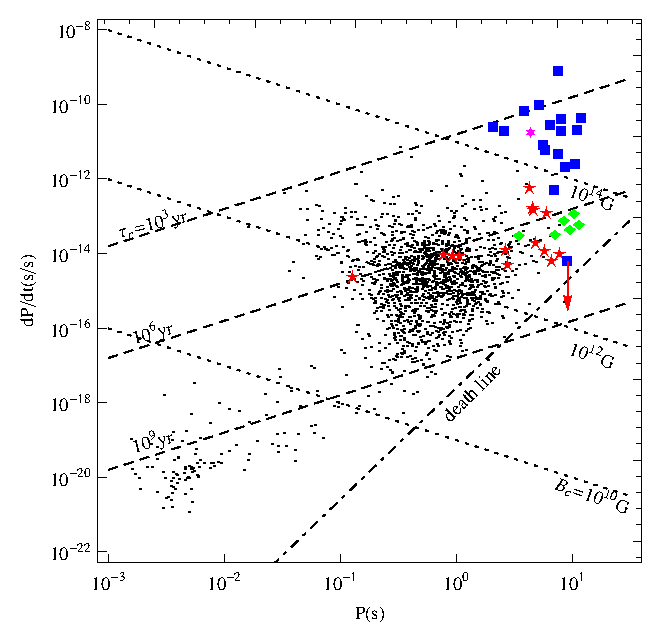
\includegraphics[width=12cm]{PPdot.eps}
\caption{脉冲星的P-$\mathrm{\dot{P}}$图\supercite{tx11}。方形点代表反常X射线脉冲星和
软伽马射线重复爆;六角星代表射电噪的磁星;向下的箭头代表低磁场的
软伽马射线重复爆(数据来自McGill online catalog:
http://www.physics.mcgill.ca/$\sim$pulsar/magnetar/main.html);
菱形代表X射线暗的孤立中子星(X-ray dim isolated neutron stars,XDINSs)
(数据来自Kaplan \& van Kerkwijk (2011)\supercite{kv11});星形代表转
动射电暂现源(rotating radio transients,RRATs);点代表常规脉冲星
和毫秒脉冲星(数据来自ATNF: http://www.atnf.csiro.au/research/pulsar/psrcat/)。}
\label{PPdot}
\end{figure}

AXPs和SGRs的自转周期分布在一个比较窄的范围内($2-12$\,s),
并且自转周期的导数与射电脉冲星比起来比较大(见图\ref{PPdot})。但是我们也发现了
自转周期导数比较小的SGR 0418$+$5729\supercite{ret10}。
%
AXPs的测时噪声远大于射电脉冲星,而SGRs的测时噪声甚至
更大。我们在所有有长时间测时数据的AXPs中都观测到了周期跳变现象(glithes)。
大多数AXPs的跳变现象和年轻射电脉冲星的相似,这暗示AXPs和
SGRs是比较年轻的脉冲星。然而,他们的跳变的幅度比有相似自转周期的射电
脉冲星更大,发生的频率也更高。跳变的起源仍然不清楚,但是所观测到的各种现象似乎
跟AXPs和SGRs的星震模型更加符合\supercite{m08}。
%
另外一个有趣的发现是在SGRs的巨爆发的尾巴中的准周期振荡(quasi 
periodic oscillations,QPOs)现象。这个现象最初是被RXTE卫星在SGR 1806$-$20在
2004年12月27日的巨爆发的尾巴中发现的\supercite{ibs05},并且被RHESSI卫星
独立地确认\supercite{ws06}。在RXTE的SGR 1900$+$14在1998年8月的巨爆发的数据
中也找到了准周期振荡现象\supercite{sw05}。这种在巨爆发的尾巴中发现的准周期振荡
现象很可能源自于由剧烈的爆发导致的星体壳层的碎裂和震动,与地球的地震相似\supercite{m08}。

\subsection{磁星模型和“夸克星+回落盘”模型}

AXP和SGRs的研究的一个最根本的问题是持续X射线辐射
和爆发现象的能源机制。AXPs和SGRs的爆发现象的能量达到
$10^{42}$\,$\rm{erg\ s^{-1}}$的量级,远大于自转所能提供的能量。一种可能的解释
是这些孤立中子星是由磁场供能的,这种模型叫做磁星模型。在磁星模型下,AXPs和SGRs
都是由极强的磁场供能的,磁场强度达到$3\times10^{17}\times(1\ \rm{ms}/P_{\rm{0}})$。
这样的极强磁场是由非常高效的发电机机制产生的,并且假设中子星在诞生时的自转
周期足够短($P_{\rm{0}}\sim1-2$\,ms),同时还有对流的存在\supercite{td93}。
由于很强的偶极辐射,磁星的自转减慢非常大,而很窄的自转周期的分布则解释为
年轻的磁星很快的自转减慢到几秒,然后快速演化到“死亡线”以下。随着自转减慢,
磁场能量,$E_{\rm{mag}}\sim10^{46}(P/5\ \rm{s})(\dot P/10^{-11}\ \rm{s\ s^{-1}})$ ergs,
很快超过自转能损\supercite{m08}。磁场的衰减提供了巨大的内部的加热,从而
产生持续的X射线辐射。而爆发现象则被解释为磁重连\supercite{td93}。

尽管磁星模型得到了深入的发展并且被广泛使用,但是随着观测的不断积累越来越多的
问题被暴露出来。我们没有发现磁星模型预测的很大的kick速度\supercite{hcb+07}和
高能量的超新星爆发\supercite{gsg+01,vk06}。我们也没有观测到AXPs和SGRs的
伽马射线辐射\supercite{tsx11}。
%
因此,不同于磁星模型的解释是有必要的,并且很有希望可以更好地解释观测。
“夸克星+回落盘”就是一个能解释我们观测到的各种AXPs和SGRs的现象的模型。
超新星爆发抛出的一些物质可能会回落到中子星周围,如果
这些回落物质带有角动量,那么它们将形成中子星周围的回落盘。AXPs
和SGRs的自转周期的分布可以解释为当共转半径等于磁层半径时达到
的回落盘的平衡周期,而回落盘的制动可以解释比射电脉冲星大的自转周期的减慢\supercite{a01,chn00}。
AXPs和SGRs的持续X射线辐射可以通过吸积过程产生,
而爆发现象则解释为夸克星的引力能、弹性能以及相变能的释放\supercite{tx11}。
夸克星还能解释超爱丁顿光度的爆发现象,因为夸克星是由强相互作用束缚的。

\subsection{反常X射线脉冲星和软伽马射线重复爆的硬X射线辐射}

AXPs和SGRs的硬X射线辐射的发现相较于软X射线
辐射是比较晚的。考虑到它们在10\,keV以下比较软的谱,所发现的一直延伸
到150\,keV的硬X射线辐射让人比较惊讶\supercite{khm04,mcl+04,dhk+06}。
到目前为止,20\,keV以上的硬X射线辐射已经在五颗AXPs
(4U 0142$+$61,1RXS J1708$-$40,1E 1048$-$59, 1E 1841$-$045,1E 1547$-$54)\supercite{dhk+06,khd+06,lwr08,khm04,enm+10}
以及两颗SGRs(SGR 1900$+$14, SGR 1806$-$20)\supercite{gmt+06,emt+07}
中发现。对于没有探测到硬X射线辐射的源,目前给出的上限也不足以排除硬
X射线辐射存在的可能性。AXPs在20\,keV以上的谱能用一个比较硬
的幂律谱拟合,而SGRs的硬X射线谱要更陡。更重要的是,在
X射线波段的比较硬的谱说明在这个波段释放的能量占了总能量的很大
一部分\supercite{m08}。

我们还不能很好地理解AXPs和SGRs的硬X射线辐射的
起源。一方面,目前的观测被硬X射线望远镜较低的灵敏度限制。另一方面,
理论模型还有待发展。在磁星模型的框架下,人们提出了几种可能的辐射机制。
Thompson \& Beloborodov (2005)\supercite{tb05}给出了两种机制,一种
机制认为硬X射线辐射是由星体表面的、薄的湍流层产生的韧致辐射,另一种机制是在星体
表面以上约100公里的高度的同步辐射。第一种辐射机制预言硬X射线谱在
几百keV会出现截断,而第二种辐射机制则预言硬X射线辐射会一直延伸到1\,MeV
甚至更高能。Heyl \& Hernquist (2005)\supercite{hh05}根据fast-mode 
breakdown模型提出,硬X射线是由在磁层外部的非热的正负电子的回旋辐射
产生的。Baring and Harding (2007)\supercite{bh07}提出,共振回旋
散射(resonant cyclotron scattering,RCS)是产生硬X射线辐射的机制。
考虑到磁层中的等离子体的密度很高,同时磁场很强,康普顿散射会在
回旋能量产生共振,从而大大增加散射截面。由星体表面辐射出的热光子
被共振回旋散射到硬X射线的能量。这个模型预言一个很平的、延伸到极高能的谱。
在回落盘的模型下,软X射线和硬X射线辐射都被解释为由吸积过程产生的。
幂律的硬X射线谱是在吸积流中由于整体康普顿化(bulk-motion Comptonization)
的光子产生的,而这些光子来自星体表面的热辐射。使用这一模型,
Tr\"{u}mper et al. (2010)\supercite{tze+10}成功地模拟了AXP 4U 0142$+$61
的软X射线和硬X射线谱。

\begin{figure}
\begin{center}
\includegraphics[width=2 in,angle=-90]{10ms_comptb_po.ps}
\includegraphics[width=2 in,angle=-90]{1ms_comptb_po.ps}
\caption{AXP 4U 0142$+$61的模拟硬X射线谱。左图曝光时间为$10^7$\,s,
右图曝光时间为$10^6$\,s。红色的点和线代表共振回旋辐射模型,黑
色的点和线代表整体康普顿化模型。}
\label{10ms}
\end{center}
\end{figure}

\begin{figure}
\centering
\includegraphics[height=0.45\textwidth, angle=-90]{1708spe.eps}
\includegraphics[height=0.45\textwidth, angle=-90]{1547spe.eps}\\
\includegraphics[height=0.45\textwidth, angle=-90]{1806spe.eps}
\includegraphics[height=0.45\textwidth, angle=-90]{0501spe.eps} \\
\caption{四颗反常X射线脉冲星/软伽马射线重复爆的$E^2f(E)$。最佳的整体康普顿化
模型的拟合结果和拟合的參差也分别给出。Suzaku XIS和INTEGRAL IBIS-ISGRI数据分别用
黑线和红线表示。}
\label{bmc}
\end{figure}

尽管对于AXPs和SGRs的硬X射线辐射的研究
受限于目前的硬X射线望远镜较低的灵敏度,但是这种状况很快会随着
下一代望远镜(例如NuStar和HXMT)的运行而得到改变。硬X射线波段观测的灵敏度
的显著提高有望帮助我们区分不同的辐射模型,从而进一步理解AXPs和SGRs
的本质。我们通过模拟AXPs和SGRs的硬X射线谱,研究了未来使用HXMT区
分不同辐射模型的可能性。我们主要考虑了两种辐射模型,一种
是磁星模型下的共振回旋辐射机制,一种是回落盘模型下的整体康普顿
化机制。这两种辐射机制预言了非常不同的硬X射线谱。共振回旋辐射
预言了一个延伸到MeV的很平的谱,而整体康普顿散射模型则预言硬
X射线谱会在200\,keV附近截断。使用HXMT的响应矩阵,
我们基于以上两种模型模拟了AXP 4U 0142+61的硬X射线能谱。我们
的模拟显示,未来HXMT的观测很有希望区分这两种模型。
在图\ref{10ms}中,我们假设$10^7$\,s和$10^6$\,s的曝光时间模拟
了AXP 4U 0142+61的能谱。我们可以看到HXMT在硬X射
线波段的高灵敏度能清楚地显示整体康普顿化模型在200\,keV预言的截断,
而共振回旋辐射的能谱则一直延伸到高能。

除了进行模拟,我们也使用了现有的数据来检验回落盘模型框架
下的整体康普顿化机制。Guo,\textbf{Dai} et al. (2015)\supercite{gdl+14}
使用Suzaku和INTEGRAL卫星的数据研究了四个源的软X射线和硬X射线辐射
(1RXS J170849$-$400910,1E 1547.0$-$5408,SGR 1806$-$20,SGR 0501$+$4516)。
我们的结果显示,这四个源的软X射线和硬X射线谱都能比较好的被整体
康普顿化模型拟合,说明回落盘模型是可以解释AXPs和SGRs的X射线辐射的。

%\section{夸克星相变潜热作为伽玛射线暴余辉能量注入的研究}
%
%冷夸克物质的费米能远高于热能,主要的自由度是夸克自由度,它们的物态至今仍不能很好理解,
%这一方面是由于在低能下夸克之间的强相互作用的非微扰效应,另一方是由于多体问题的困难。
%中子星作为最致密的一种天体之一,其中心的密度高达几倍核物质密度,这无疑为我们提供了一个
%研究夸克物质物态的绝佳场所。有相对论重离子碰撞实验的证据显示,在热夸克胶子等离子体中,
%夸克间的相互作用很强\supercite{Shuryak09},那么自然地当温度降低时,夸克之间的相互作用
%可能更强。相对论性的夸克物质基态可能不是费米气\supercite{Xu09},于是夸克可能集团,
%而如果夸克团块之间的剩余强相互作用势能高于它们的动能,则夸克团块将被束缚在势垒中,
%形成固态夸克物质,我们推测天体物理中的冷夸克物质可能处于这样的固态\supercite{Xu03}。
%
%由于目前我们尚不能得到冷夸克物质的相对论性状态方程,通常只能使用一些唯象模型来描述,
%Lai \& Xu (2009)使用了~Lennard-Jones~势来讨论固态夸克星\supercite{Lai09},得到了夸
%克星的状态方程。基于Lai \& Xu (2009)的固态夸克星模型,我们可以尝试估算夸克星从液态
%相变到固态时放出的相变潜热以及相变温度,并将估算结果应用于伽玛暴余辉平台的解释。
%
%
%假设夸克星内部的单个夸克团块是不带色的,于是我们可以将夸克星内部的夸克团块与惰性气体
%中电中性的的惰性气体分子类比。我们知道惰性气体分子之间的相互作用能很好地用~Lennard-Jones~势来刻画:
%\begin{equation}
%u(r)=4U_{0}[(\frac{r_{0}}{r})^{12}-(\frac{r_{0}}{r})^{6}]
%\end{equation}
%其中,$U_{0}$ 是势井深度,$r_{0}$ 代表相互作用的范围。我们假设这样一个短程排斥,
%长程吸引的相互作用势也能描述夸克团块之间的相互作用,那么当夸克团块间的相互作用势井足
%够深,以至于能将夸克团块束缚于势垒内时,夸克物质就将固化,形成固态夸克物质。由于
%色相互作用远远强于电磁相互作用,$U_{0}$ 和 $r_{0}$ 两个参数在冷夸克物质中将会不同
%于惰性气体中,并且决定了固态夸克物质的状态。用~Lennard-Jones~势来刻画的固态夸克星模型
%完全不同于用~MIT bag model~等模型来刻画的夸克物质模型。相比于在传统模型中夸克物质
%的基态是费米气,在~Lennard-Jones~势所描述的固态夸克星模型中,夸克团块是非相对论性
%的粒子,并且预言了一个更硬的状态方程,意味着夸克星的最大质量将更大($>2M_{\odot}$)。
%
%基于用~Lennard-Jones~势来描述的固态夸克星模型,我们可以尝试估算夸克星由液态相变到
%固态的过程中放出的相变潜热及相变温度。这样的相变过程有可能发生在夸克星形成的初期,
%当夸克星由高温逐渐冷却时,例如我们将讨论的伽玛暴余辉阶段。在我们所考虑的固态夸克星
%模型下,夸克团块作为非相对论性粒子,由之间的类似于~Lennard-Jones~势的剩余色相互作用
%束缚在一起,与惰性气体非常相似,与常见的物质也有很多相似之处。鉴于我们很难从分子动
%力学的方法直接出发,模拟夸克物质从液态相变到固态的过程,并得到相变潜热和相变温度,
%我们考虑通过与惰性气体,以及常规物质的类比,尤其是参考各种物质的相变潜热和
%相互作用强度的数据,从量级上估算夸克星由液态相变到固态时释放的相变潜热,这对于我们
%讨论伽玛暴余辉的能量注入是十分有意义的。在表\ref{heat}中,我们列出了一些常见物质
%和惰性气体的熔解热,气化热,势能以及势能与熔解热之比的实验数值,其中熔解热正对应于
%从液态相变到固态的相变潜热,而势能的数值对于有升华热数据的物质就是升华热,对于没
%有升华热数据的物质则是熔解热和气化热之和。我们看到,对于大部分物质,包括惰性气体,
%势能与熔解热之比在几十到一百之间,特例是氦的比值较高,这可能与氦复杂的物态有关。考
%虑到夸克团块间的相互作用与惰性气体相似,且夸克团块的质量不大,我们取势能与熔解热之比
%为$20\sim100$进行估算。而在之前讨论的固态夸克星模型下,取势井深度$U_{0}=100$\,MeV,
%那么我们可以估算得到单个夸克团块由液态相变到固态是放出的相变潜热为$1\sim5$\,MeV。假
%设夸克星的质量是一个太阳质量,$M_{\odot}\approx2\times10^{33}$\,g,约包含重子数目为
%$10^{57}$个,这样我们得到一个太阳质量的夸克星由液态相变到固态放出的相变潜热约为$E\approx10^{51}$\,ergs,
%这个估算值基本上就是伽玛暴余辉释放能量的典型值,也就是说夸克星由液态相变到固态时释
%放的相变潜热完全足够提供伽玛暴余辉平台需要的能量注入。
%						
%\begin{table}[htb!]
%\caption{一些常见物质和惰性气体的熔解热,气化热,势能以及势能与熔解热之比}
%\label{heat}
%\centerline{\begin{tabular}{lccccc}\hline
%	&  熔解热 kcal/mol  & 气化热 kcal/mol   & 势能 kcal/mol  &   势能/熔解热  \\
%\hline
%$He$ & 0.0033 & 0.0194 & 2.2944   & 695.27 \\
%$Ne$ & 0.0801 & 0.422  & 9.1776   & 114.58 \\
%$Xe$ & 0.5495 & 3.02   & 12.6192  & 22.96  \\
%$Rn$ & 0.69   & 4.01   & 19.5024  & 28.26  \\
%&        &        &          &        \\
%$Al$ & 2.56   & 69.5   & 78       & 30.47  \\
%$Cs$ & 0.499  & 16.198 & 18.3     & 36.67  \\
%$Cu$ & 3.17   & 72.74  & 81       & 25.55  \\
%$Fe$ & 3.63   & 83.68  & 99.5     & 27.41  \\
%$Hg$ & 0.5486 & 14.13  & 14.65    & 26.7   \\
%$Na$ & 0.622  & 23.285 & 25.75    & 41.4   \\
%$Si$ & 12     & 85.8   & 107.7    & 8.98   \\
%$C$  & 25     &        & 171.29   & 6.85   \\
%$CO$ & 0.2    & 1.444  & 1.644    & 8.22   \\
%$CO_{2}$  & 1.99      &        & 6.03   & 3.03  \\
%$H_{2}O$  & 1.436      &  9.717    & 11.153   & 7.77  \\
%$H_{2}O_{2}$  & 2.987   &  10.53   & 12.34   & 4.13   \\
%$CaCl_{2}$  & 6.8      & 56.2       & 77.5   & 11.4  \\
%\hline
%\end{tabular}}
%\end{table}
%
%另一方面,根据~Lindemann~经验定则,当固体中原子振动强度的方均根与平衡的相
%邻原子距离的比值大于一定的临界值时固体熔解\supercite{Lindemann10},我们可以
%估算夸克星相变的温度。~P. Mohazzabi~和~F. Behroozi~在~1987~年的工作中得到,
%对于惰性气体,原子振动强度的方均根与平衡的相邻原子距离的比值有表达式:
%\begin{equation}
%\frac{\langle u^{2} \rangle}{R_{0}^{2}}=\frac{\varepsilon_{0}/kT}{4(\exp(-\alpha/kT)-\exp(-\varepsilon_{0}/kT))}\int_{\alpha/\varepsilon_{0}}^{1}[(1-x^{1/2})^{-1/6}-(1+x^{1/2})^{-1/6}]^{2}\exp(-\varepsilon_{0}x/kT)/\rm{d}x
%\end{equation}
%其中$x=1+(\varepsilon/\varepsilon_{0})$,$\varepsilon_{0}=U_{0}S_{6}^{2}/6S_{12}$,
%$k$是玻尔兹曼常数,对于简单的面心立方晶体,$S_{6}=14.45392$,
%$S_{12}=12.13188$\supercite{Moha87},带入惰性气体的参数后发现比值很好地与
%经验定则符合。对于我们的估算,可以直接参考惰性气体以及普通物质的势能与
%热能的比值,$\Gamma=U_{0}/kT$,从而估算夸克星相变的温度。表\ref{temp}列出了
%惰性气体的相关参数,可以发现,势能与热能的比值大约在$1.75$左右。而对于其他
%物质,例如对于单一组分的等离子体,液体固化时库伦势与热能的比值是$\Gamma\approx175$\supercite{DeWitt01},
%对于混合组分的等离子体,$\Gamma\approx233$\supercite{Horowitz07}。因此,
%若取势井深度$U_{0}=100$\,MeV,我们可以直接估算得到夸克星的相变温度大约在$1\sim10$\,MeV。
%\begin{table}[htb!]
%\caption{惰性气体的相变温度和势能}
%\label{temp}
%\centerline{\begin{tabular}{lccc}\hline
%	&  熔点 K  & $U_{0}/\rm{k}$ K   & $U_{0}/\rm{k}T$  \\
%\hline
%$Ne$ & 24.5 & 45.86  & 1.87 \\
%$Ar$ & 83.8 & 142.095   & 1.70  \\
%$Kr$ & 115.8   & 201.9   & 1.74  \\
%$Xe$ & 161.4   & 281.0   & 1.74  \\
%\hline
%\end{tabular}}
%\end{table}
%
%处在液态到固态相变过程中的夸克星将保持稳定的相变温度,同时向外辐射相变
%潜热,我们假设夸克星的热辐射是一个灰体辐射,辐射效率是$\eta\ll1$,则我
%们可以估算夸克星辐射相变潜热的时标:
%\begin{equation}
%t=\frac{E}{\sigma T^{4} 4\pi R^{2}\eta}
%\end{equation}
%其中,$E=10^{51}$\,ergs,$\sigma$是~Stefan-Boltzman~常数,$R=10$\,km
%是夸克星的半径,考虑到$\eta\ll1$,带入$T\approx1$\,MeV计算可得,相变潜
%热的辐射时标$t\approx1000$\,s,这是与伽玛暴余辉的平台持续时间基本一致的。
%
%在估算了夸克星由液态相变到固态时放出的相变潜热,以及能量注入的时标之后,
%我们有必要定性地讨论一下相变潜热以怎样的方式注入伽玛暴余辉的问题。
%夸克星由液态到固态的相变过程应该发生在伽玛暴的爆发阶段之后,具体的时标依赖于夸克星形成之后的冷却过
%程,但我们可以预期,相变发生时,伽玛暴的爆发过程已经结束,原始火球已经膨胀到了很远的距离,或者已经进
%入外部介质,在夸克星表面到火球内边界或外部介质内边界之间形成了一个“真空”。由于原始火球已经将这个空间
%内的大部分重子物质带出,我们假设这个空间里的重子物质密度很低,只有原始密度的$1\% \sim 0.1\%$。
%根据我们的估算结果,夸克星相变释放的相变潜热约为$E=10^{51}$\,ergs,以灰体辐射的方式释放能量的时间约
%为$1000$\,s,于是我们可以估算得到,能流约为$L=10^{48}$\,ergs/s,相比于爆发阶段的能流小了三个量
%级,然而如果用夸克星半径$R=10$\,km 作为源的尺度来估算光深,我们可以得到:
%\begin{equation}
%\tau_{\gamma\gamma}=\frac{f_{p}\sigma_{T}FD^{2}}{R^{2}m_{e}c^{2}}=10^{13}f_{p}(\frac{D}{3000\rm{Mpc}})^{2}(\frac{F}{10^{-11}\rm{ergs/cm^{2}}})(\frac{R}{10\rm{km}})^{-2}
%\end{equation}
%可见光深仍然非常大。因此,由夸克星相变释放出的相变潜热能流仍将类似于原始火球,
%是由光子,电子对和少量重子物质构成的类似理想流体的等离子体,并且在内部压强的作
%用下加速膨胀,不同的是火球不再是以极端相对性速度朝静止观测者运动,同时由于相变
%过程相对稳定,也不会在火球内产生壳层。这样的一个由释放相变潜热形成的火球将基本
%按照我们在上一节中讨论的火球演化的过程演化,也会有由光厚到光薄的过度,以及有
%辐射主导到物质主导的过度。然而无论演化过程怎么样,我们期待最后能量将转化为
%重子物质的动能,于是我们可以简单地估算最后由重子物质主导的火球的速度:
%\begin{equation}
%\gamma=L/Mc^{2}
%\end{equation}
%我们知道在爆发阶段,$\gamma\approx100$,而如前所述,我们考虑夸克星相变潜热注
%入阶段,能流比爆发阶段小三个数量级,而重子物质质量为原始质量的 $1\%$,由此可得
%$\gamma\approx10$。而这样的相对能量密度较小的能流,以 $\gamma\approx10$的速度
%进入外部介质,根据Zhang et al. (2002)\supercite{Zhang02},能流将以类似于~Poynting~
%流的方式注入余辉。
%
%由以上的论述,我们可以大致描绘夸克星相变潜热注入伽玛暴余辉的图像,在伽玛暴的爆
%发阶段结束以后,中心形成的夸克星温度逐渐降低,当达到固化温度时,夸克星发生由液态
%向固态的相变,相变过程中温度稳定在相变温度,相变潜热则以灰体辐射的方式稳定地向外辐射;
%辐射出的光子由于能量密度很高,光深很大,产生大量电子对,而光子,电子对和少量的重子
%物质耦合在一起类似理想流体,按照爆发阶段火球演化相类似的方式演化;随着火球的膨胀,
%最终能量将基本上转化为重子物质的动能,而由于潜热释放的能流较小,虽然重子物质相较
%于爆发阶段少很多,最后加速达到的速度也不是很高,而这样的能流较小,速度不高的火球
%将以类似于~Poynting~流的形式注入余辉,也就是说将能量较平和地转换给外部介质的物质,
%从而产生余辉阶段的平台;而在相变结束之后,相变潜热的注入停止,外部介质不再得到
%能量注入,辐射的流量迅速降低,从而产生光变曲线平台后的快速而陡峭的下降。

\pkuthssffaq

